\section{RESULTS}
\label{sec:results}

We have applied our Bayesian anomaly detection framework to all suitable Type Ia supernovae from the Hawaii Supernova Flows dataset \citep{do2025hawaii}. In this section, we first present a global statistical comparison between our method and the systematic approximation of traditional filter selection, before using three representative supernovae to illustrate the framework's different benefits.

\subsection{Similarity Analysis}

Our global similarity analysis confirms that the automated framework (Case C; Section~\ref{subsec:analysis_cases}) produces parameter estimates that are statistically consistent with our systematic filter selection approach (Case B; Section~\ref{subsec:analysis_cases}). The overall agreement demonstrates the reliability of our automated approach. To investigate the systematic differences observed, particularly in the colour parameter, we performed a contamination analysis (Section~\ref{subsec:contamination_analysis}) that establishes how anomalous data points correlate with both brightness and wavelength, revealing systematic patterns in the data quality that can affect parameter estimation.

The results, summarised in Figure~\ref{fig:similarity_corner}, show that 98.2 per cent of all parameter estimates agree to within 1$\sigma$ of their combined uncertainty. On an object-by-object basis, 93.9 per cent of supernovae have all four of their parameters agreeing within this 1$\sigma$ threshold. The mean normalised differences are $\Delta t_0 = 0.154\sigma$, $\Delta \log x_0 = 0.175\sigma$, $\Delta x_1 = 0.097\sigma$, and $\Delta c = 0.418\sigma$.

\begin{figure*}
\centering
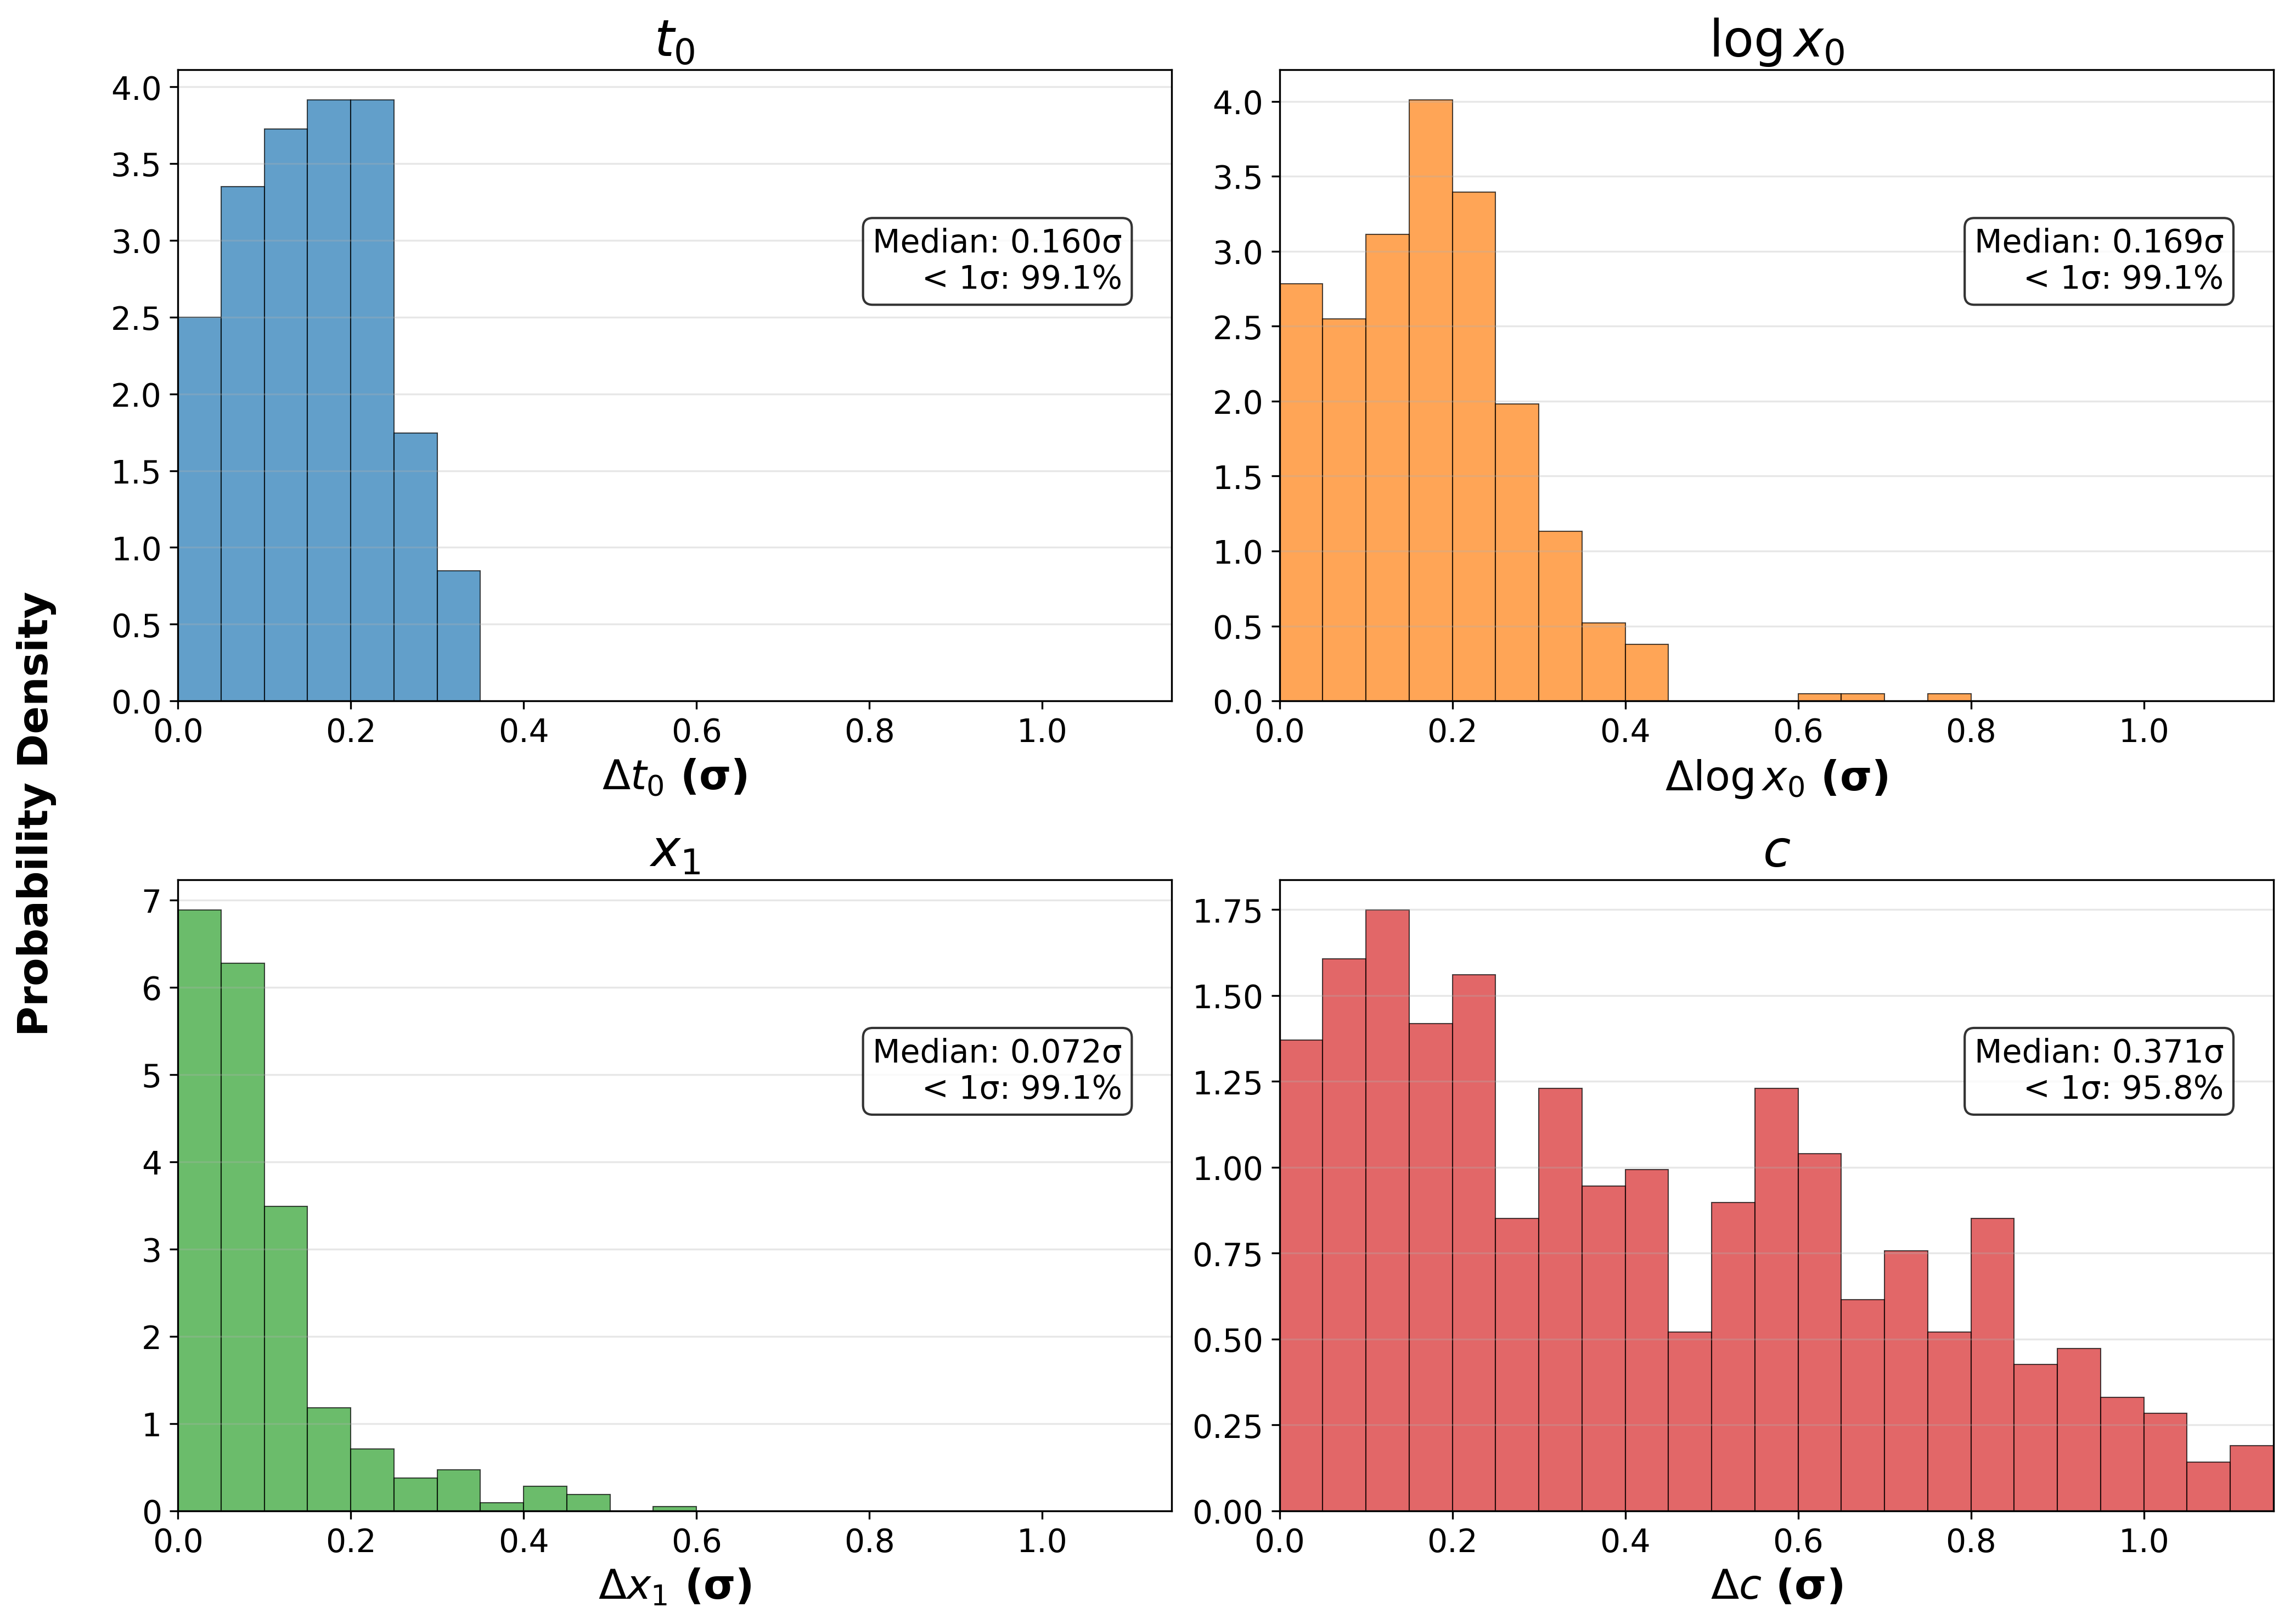
\includegraphics[width=0.8\textwidth]{images/normalized_difference_bars_Ia_all.png}
\caption{A histogram visualising the distributions of the normalised difference, $|\Delta\theta|$, for the four SALT3 parameters, comparing our anomaly detection method to the systematic filter selection approach (Case B) across all supernovae. The vast majority of the probability mass (98.2 per cent) lies well within the 1$\sigma$ similarity threshold, demonstrating that the two methods agree within their combined uncertainties. For the color parameter, the distribution is slightly more spread out with a median of 0.371$\sigma$ and 95.8 per cent of the probability mass within 1 sigma of the traditional analysis.}
\label{fig:similarity_corner}
\end{figure*}

Notably, the colour parameter $c$ (one of the SALT parameters described in Section~\ref{subsec:salt_model}), exhibits a modestly larger average difference ($\Delta c = 0.418\sigma$) than other parameters. This is interesting because it indicates a systematic difference in our method's predictions versus traditional methods' predictions. This suggests that in addition to automating the data curation process, we may be removing anomalies that are systematically influencing subsequent cosmological analyses, as quantified in our contamination analysis (Section~\ref{subsec:contamination_analysis}). By preserving valid data points in partially contaminated filters, a capability we term `filter preservation', the method retains colour information that is lost when entire bandpasses are discarded. This improvement in data retention, while small for individual objects, has the potential to significantly impact cosmological analyses of large samples by reducing biases introduced by coarse data rejection.

\subsection{Contamination Analysis}
\label{subsec:contamination_analysis}

To understand the systematic differences observed in the similarity analysis, particularly for the colour parameter, we performed a contamination analysis across the supernova sample. This analysis quantifies how anomalous data points systematically bias SALT3 parameter estimation through the contamination metrics defined in Section~\ref{subsec:contamination_quantification}.

\begin{figure*}
\centering
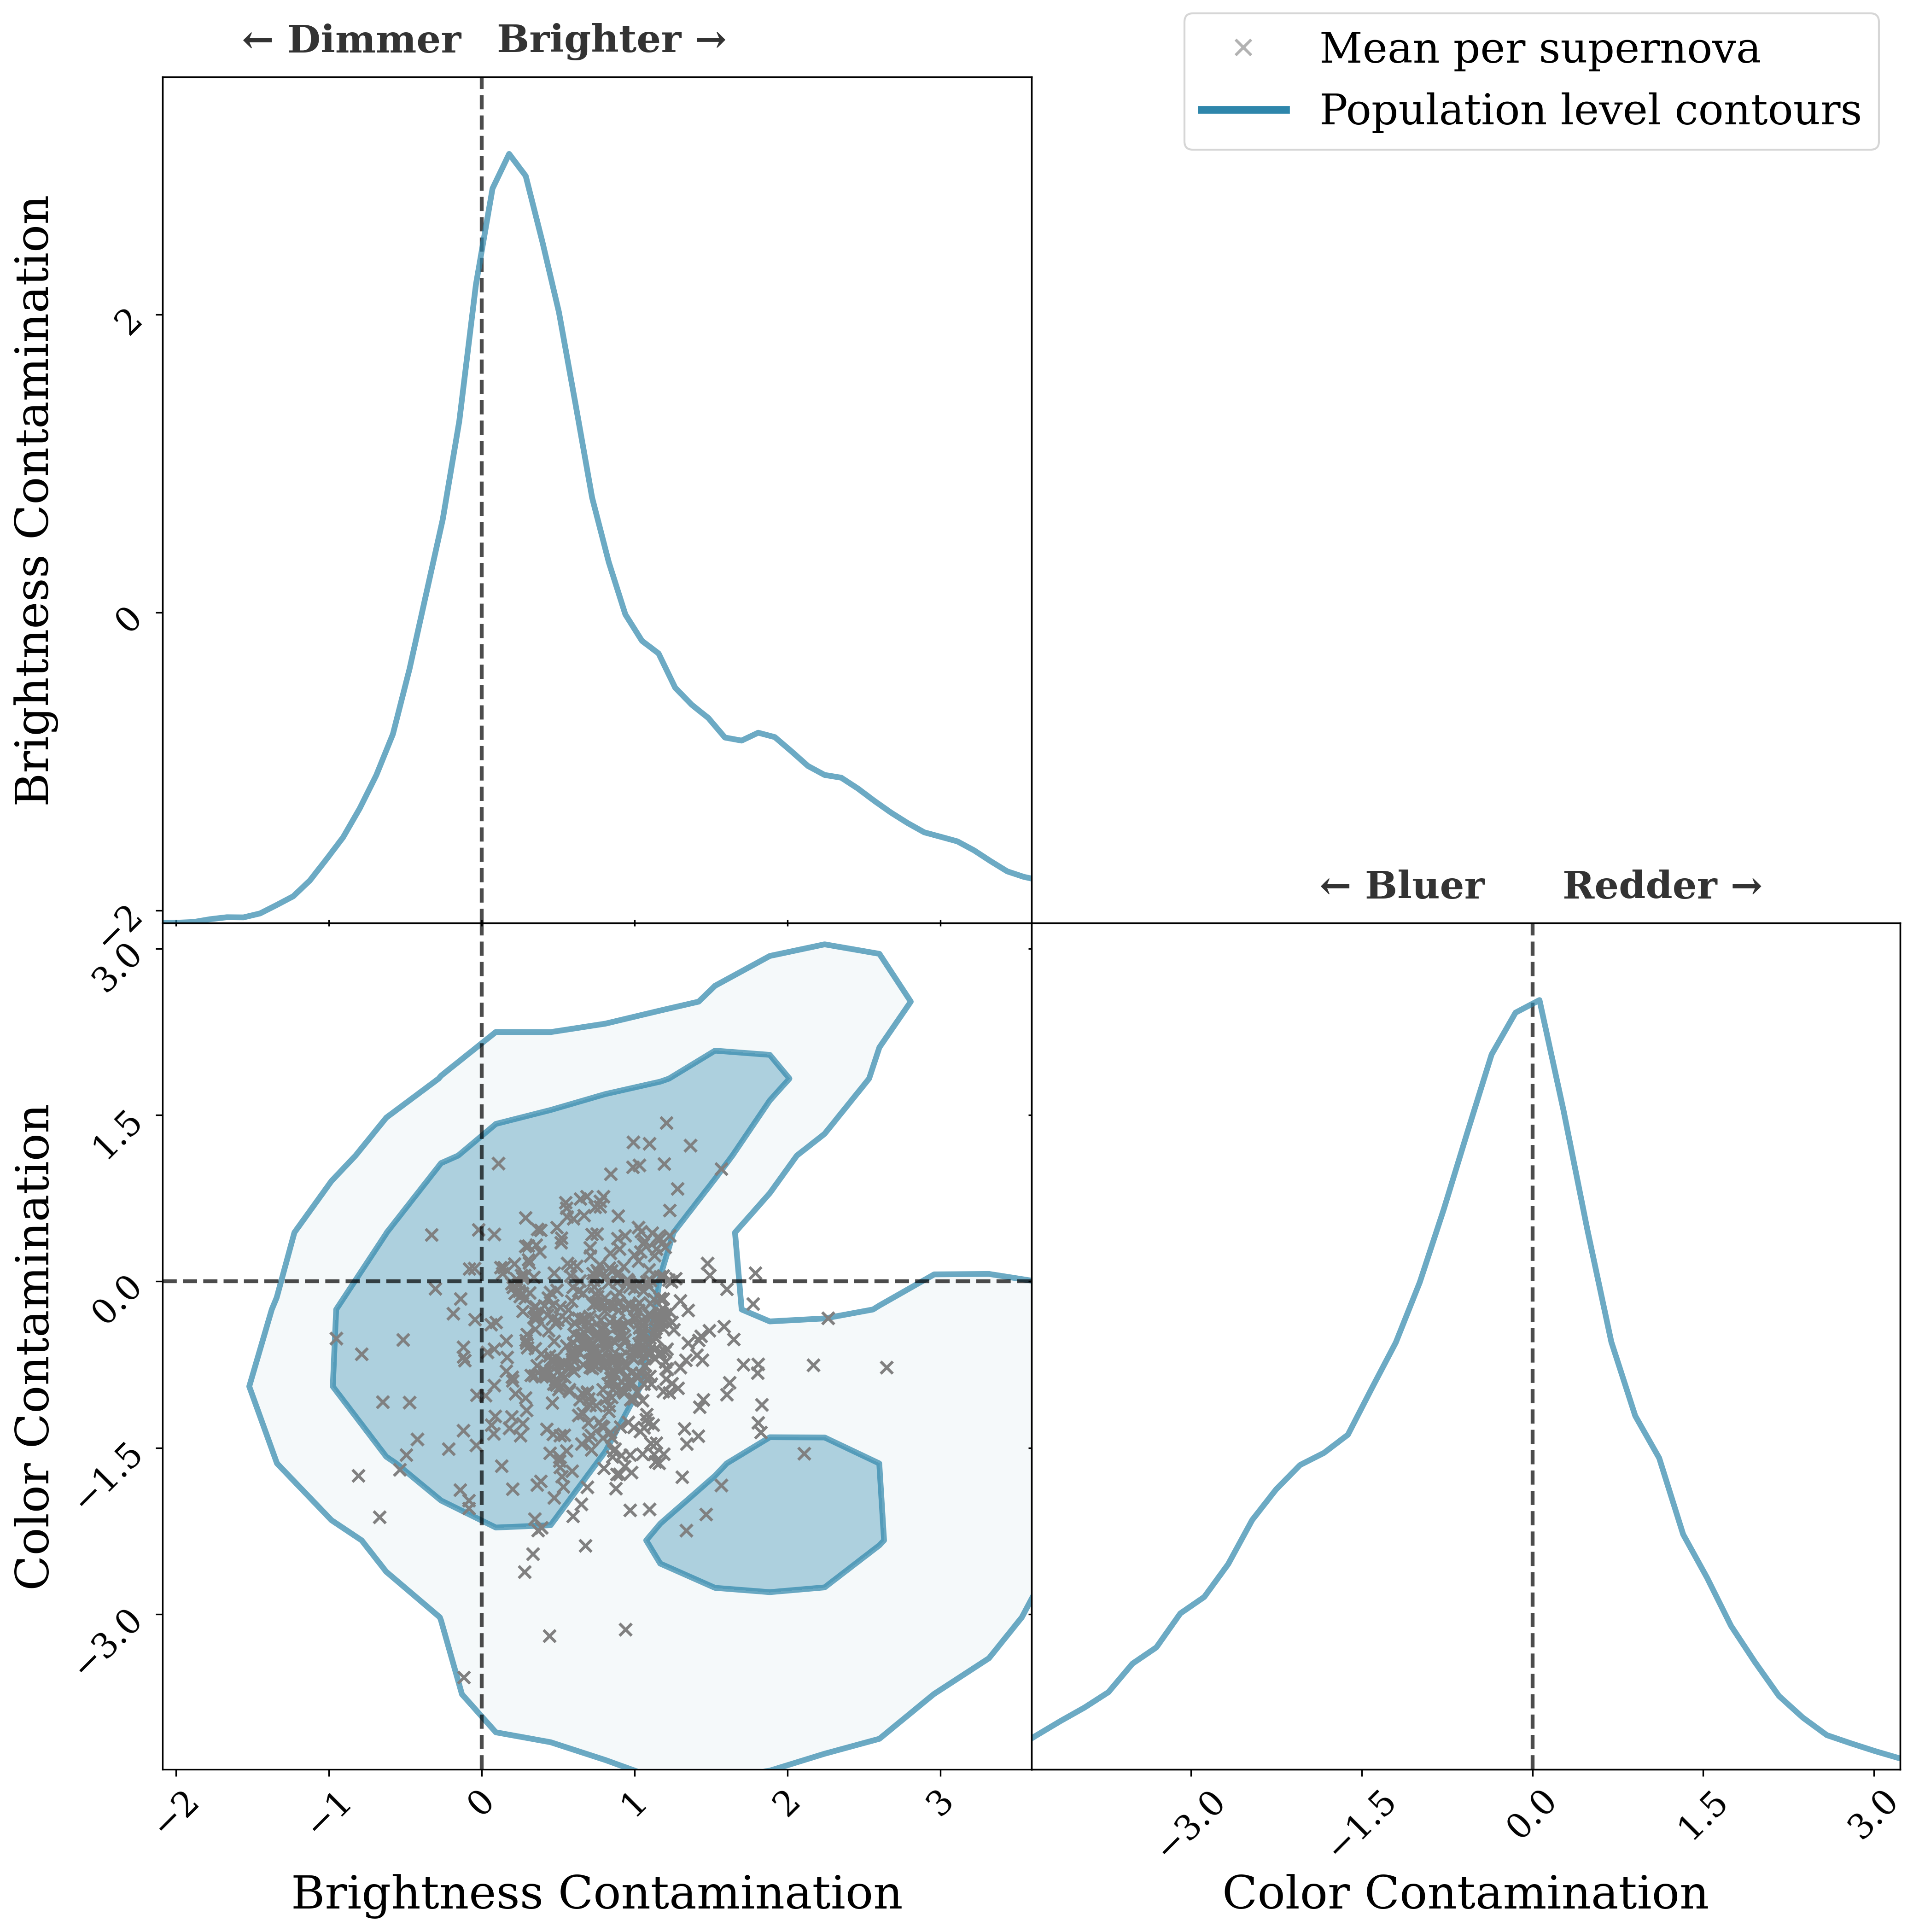
\includegraphics[width=0.8\textwidth]{images/recreated_contamination_plot.png}
\caption{Distribution of contamination metrics across the supernova sample. The diagonal panels show 1D marginal distributions for brightness contamination $C_{\mathrm{bright}}$ (top left) and colour contamination $C_{\mathrm{colour}}$ (bottom right). The bottom left panel shows the 2D joint distribution with 1$\sigma$ (inner) and 2$\sigma$ (outer) contours. Grey crosses mark individual supernova measurements. The positive mean brightness contamination and negative mean colour contamination indicate systematic biases in the anomalous data.}
\label{fig:contamination_triangle}
\end{figure*}

Figure~\ref{fig:contamination_triangle} presents the distribution of contamination metrics across the supernovae analysed. The brightness contamination $C_{\mathrm{bright}}$ showed a posterior mean of 0.718 $\pm$ 0.862 across the population, with a 1$\sigma$ confidence interval of [-0.065, 1.660]. Importantly, this contamination metric incorporates the probabilistic nature of anomaly detection: each data point contributes to the contamination score weighted by its probability of being anomalous, rather than through binary classification. The positive mean indicates that the net systematic effect of probable anomalies is to push flux measurements upward. Across all posterior samples, 63.8 per cent exhibit positive brightness contamination; this does not mean that 63.8 per cent of anomalies are bright, but rather that 63.8 per cent of the time, the probability-weighted contribution of all potentially anomalous points results in a net brightening effect. While this bias is less than 1$\sigma$ from zero and thus not definitively established, it suggests a systematic trend that, if left uncorrected in traditional analyses, could lead to underestimation of peak luminosity or overestimation of host galaxy extinction.

The colour contamination metric $C_{\mathrm{colour}}$ exhibited a posterior mean of -0.563 $\pm$ 0.989 across the population, with a 1$\sigma$ confidence interval of [-1.771, 0.207]. Like the brightness metric, this represents the probability-weighted net effect across all data points. The negative mean reveals that anomalous points preferentially affect blue bandpasses more than red ones. The posterior distribution shows 43.9 per cent of samples with negative colour contamination (where the probability-weighted effect pushes measurements bluer) versus 14.0 per cent with positive colour contamination (pushing redder), with the remainder showing negligible colour bias. Again, while the mean contamination is less than 1$\sigma$ from zero, the consistent direction of the bias across a substantial fraction of the posterior samples indicates a systematic tendency worth accounting for in precision cosmology. This blue preference in anomalous data provides insight into the systematic shifts observed in the colour parameter during the similarity analysis. When blue bands are preferentially contaminated with brighter measurements, traditional fitting methods that do not account for this contamination will infer artificially bluer supernovae (lower $c$ values), underestimating the true extinction. Through the Tripp relation ($\mu = m_B - M + \alpha x_1 - \beta c$), these systematically lower $c$ values would lead to underestimated distance moduli, making supernovae appear closer than they are and potentially biasing measurements of dark energy parameters and the Hubble constant.

The significant variation in both metrics, clearly visible in the broad posterior distributions in Figure~\ref{fig:contamination_triangle}, indicates substantial heterogeneity across the supernova sample. This heterogeneity demonstrates that contamination effects are not uniform across all supernovae but vary substantially from object to object. Some supernovae show strong blue contamination while others show red contamination, emphasising that our framework's ability to quantify these effects individually for each supernova is crucial. A blanket correction approach would fail to capture this diversity and could introduce new biases.

The contamination analysis provides quantitative evidence that the systematic differences between our anomaly detection framework and traditional methods, particularly the 0.418$\sigma$ average difference in the colour parameter, arise from the proper treatment of wavelength dependent contamination. By identifying and downweighting anomalous measurements that are preferentially blue and bright, our framework recovers more accurate colour parameters that better reflect the true supernova properties. This improved accuracy in individual supernova parameters will propagate through to more reliable cosmological constraints when these measurements are used for distance determinations in future analyses.

\subsection{Demonstrating the Framework: Case Studies}

Having established the global statistical performance, we now use three representative supernovae to demonstrate how the framework addresses different challenges in photometric data processing. The cases show: standard contamination mitigation via isolated outlier flagging (SN 21lnf, Section~\ref{subsec:sn21lnf}); automatic filter removal for systematically corrupted bandpasses (SN 21hwx, Section~\ref{subsec:sn21hwx}); and filter preservation, where only specific anomalous points are flagged within a bandpass (SN 19ekb, Section~\ref{subsec:sn19ekb}). For each case, we present both posterior distributions and light curve fits to compare our method with approaches that do not use automated anomaly detection.

\subsection{SN 19ekb: Filter Preservation and Tighter Constraints}
\label{subsec:sn19ekb}

The analysis of SN 19ekb illustrates the effect of filter preservation on parameter constraints. Figures~\ref{fig:19ekb_corner} and \ref{fig:19ekb_lightcurves} compare the posterior distributions for the SALT parameters from the three analysis cases. The naive fit (Case A; Section~\ref{subsec:analysis_cases}), which uses all data, yields tightly constrained but systematically biased posteriors, particularly for the colour parameter, $c$. The systematic filter selection approach (Case B; Section~\ref{subsec:analysis_cases}), in which the entire ZTF g and ATLAS c bands were removed based on our $\chi^2$ criterion, produces posteriors that are robust to this contamination, albeit with broader constraints.

In the anomaly detection framework (Case C; Section~\ref{subsec:analysis_cases}), the model automatically identifies and flags only the few anomalous points within the ZTF g and ATLAS c bands. By preserving the majority of valid data in these filters, Case C recovers parameter means consistent with the systematically cleaned data of Case B while achieving demonstrably tighter posterior constraints. This result shows that by retaining additional valid data, the framework can produce more precise parameter constraints compared to an analysis where entire filters are removed. This demonstrates that by retaining statistically valid data, our framework can improve the precision of supernova standardisation, which in turn could lead to tighter constraints on cosmological parameters that are crucial for addressing discrepancies such as the Hubble tension.

\begin{figure*}
\centering
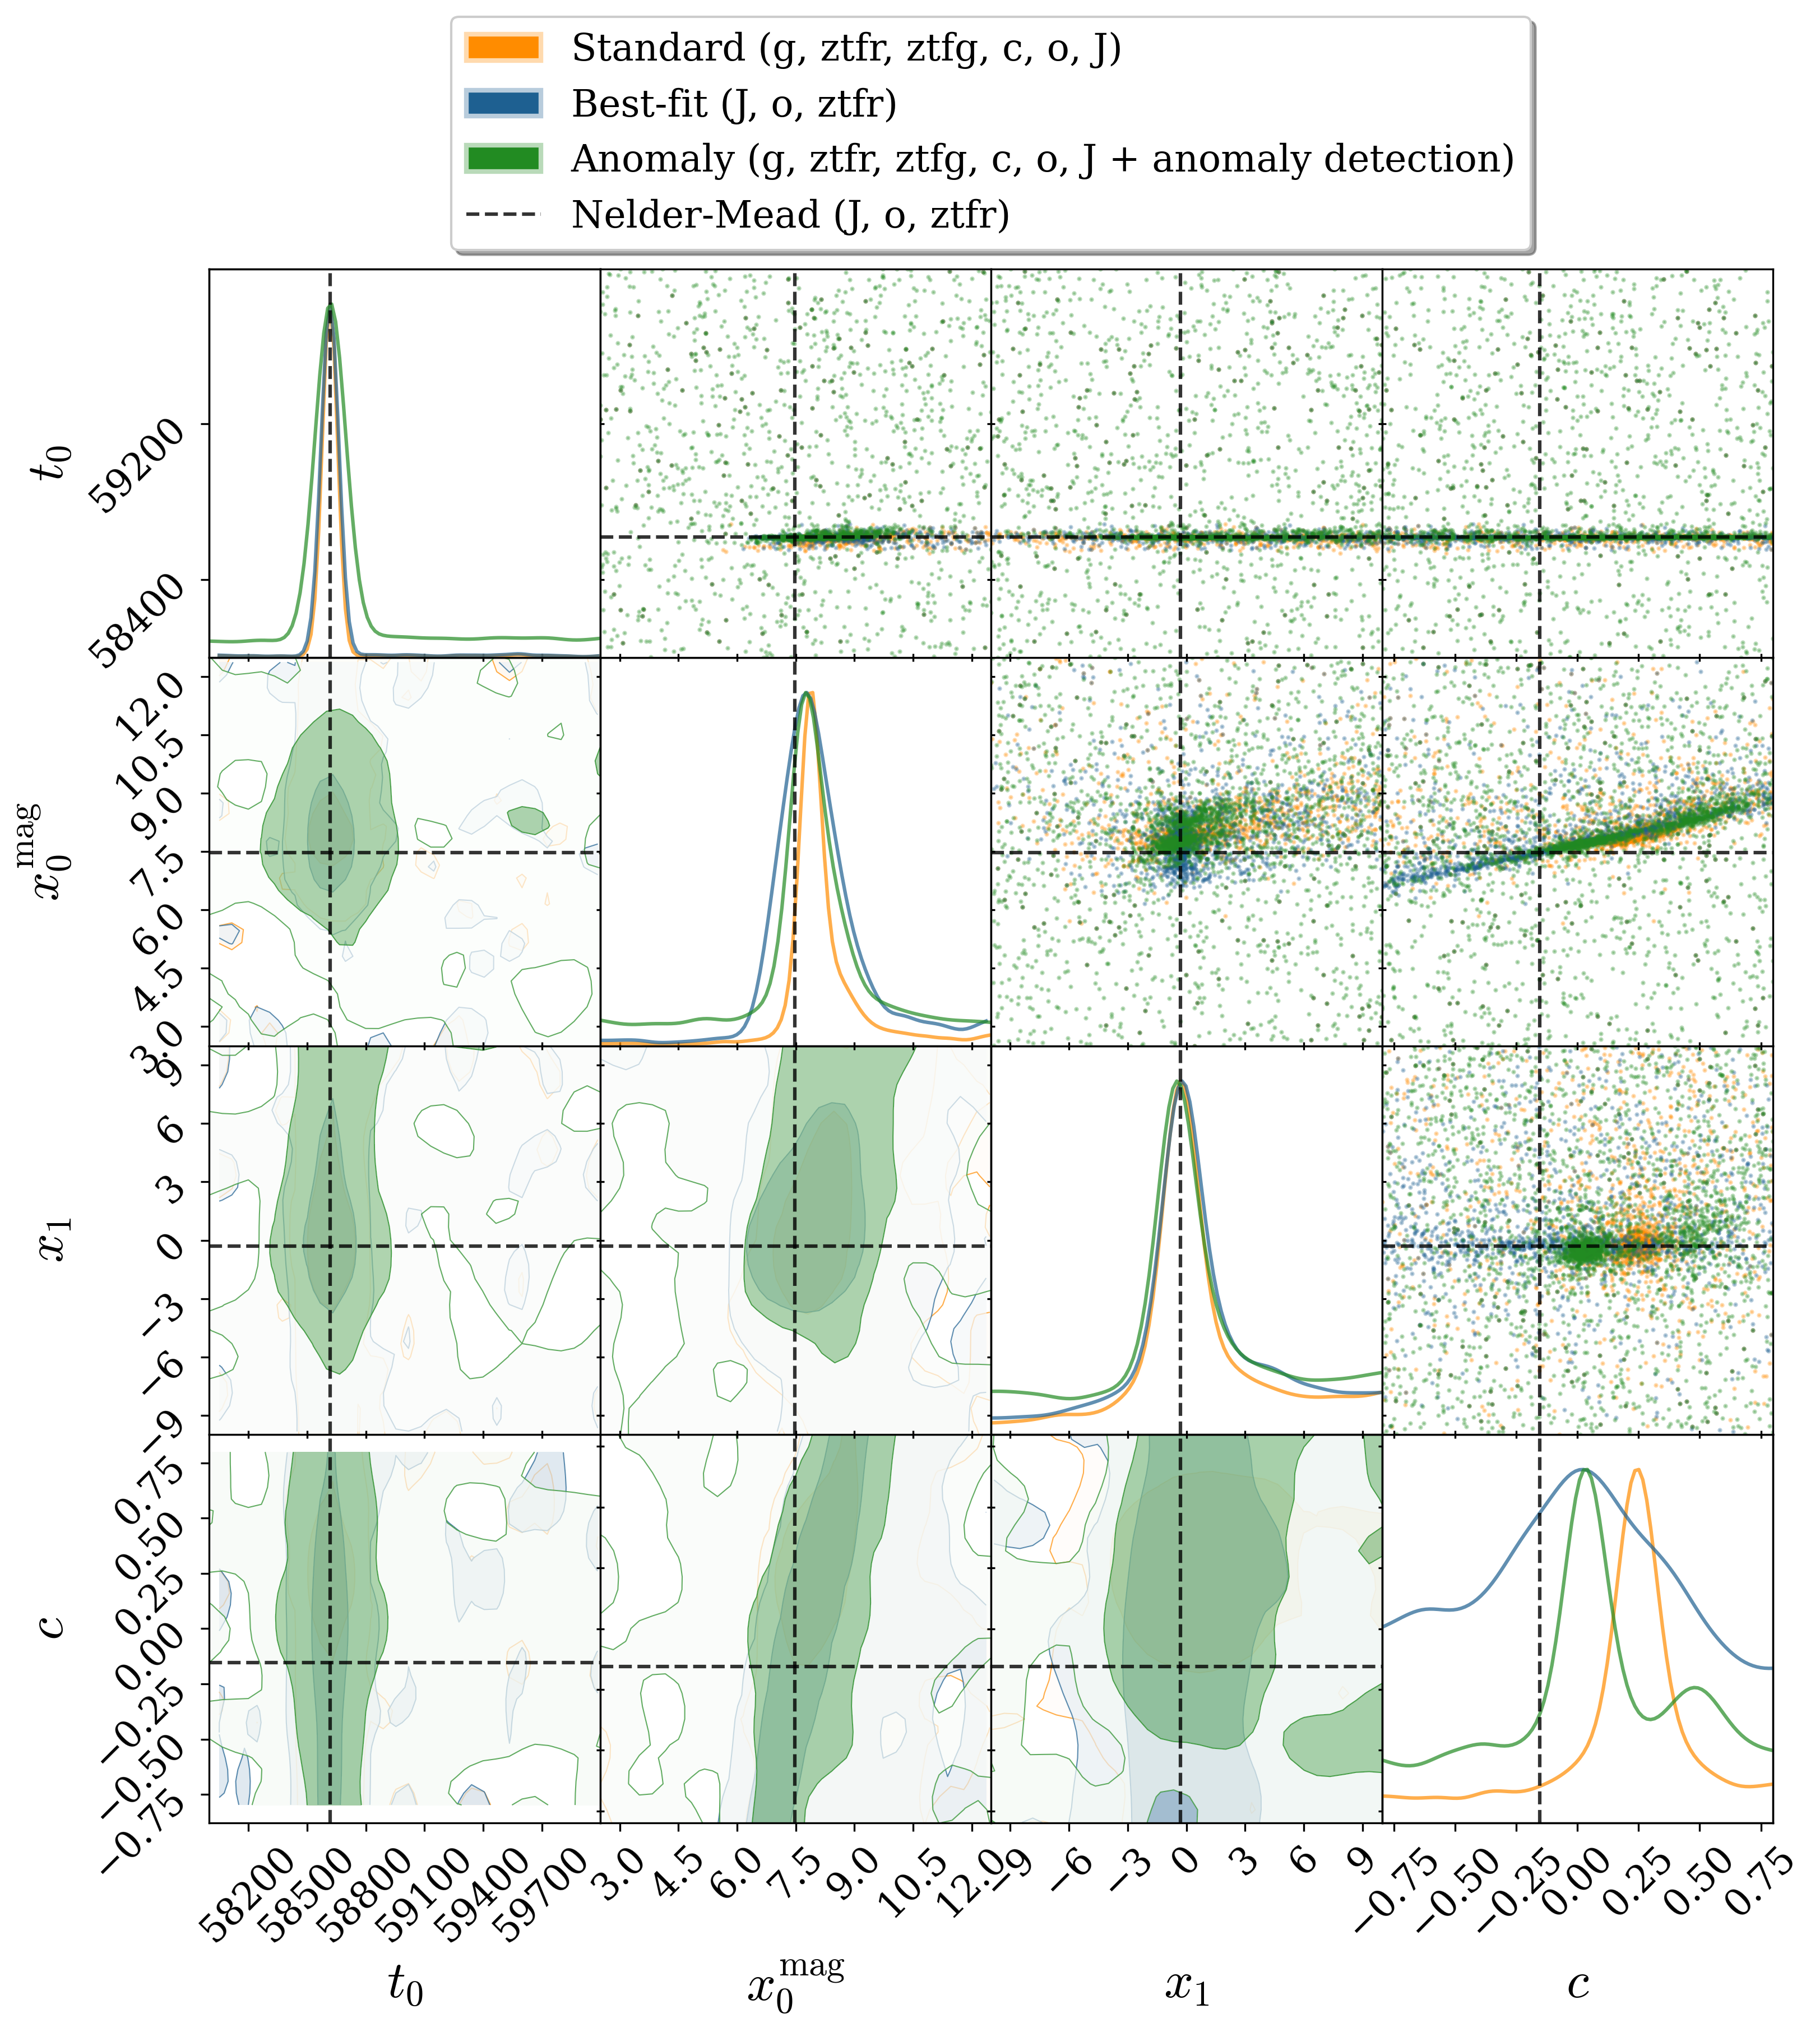
\includegraphics[width=0.8\textwidth]{images/corner_comparison_19ekb_paper_quality.png}
\caption{Corner plot showing posterior distributions for SALT parameters $x_0$, $x_1$, and $c$ for SN 19ekb. Blue contours show the naive fit using all data (Case A), orange shows the systematic filter selection with removed filters (Case B), and green shows our Bayesian anomaly detection results (Case C). The anomaly detection achieves posteriors with tighter constraints by selectively removing outliers while preserving valid data.}
\label{fig:19ekb_corner}
\end{figure*}

\begin{figure*}
\centering
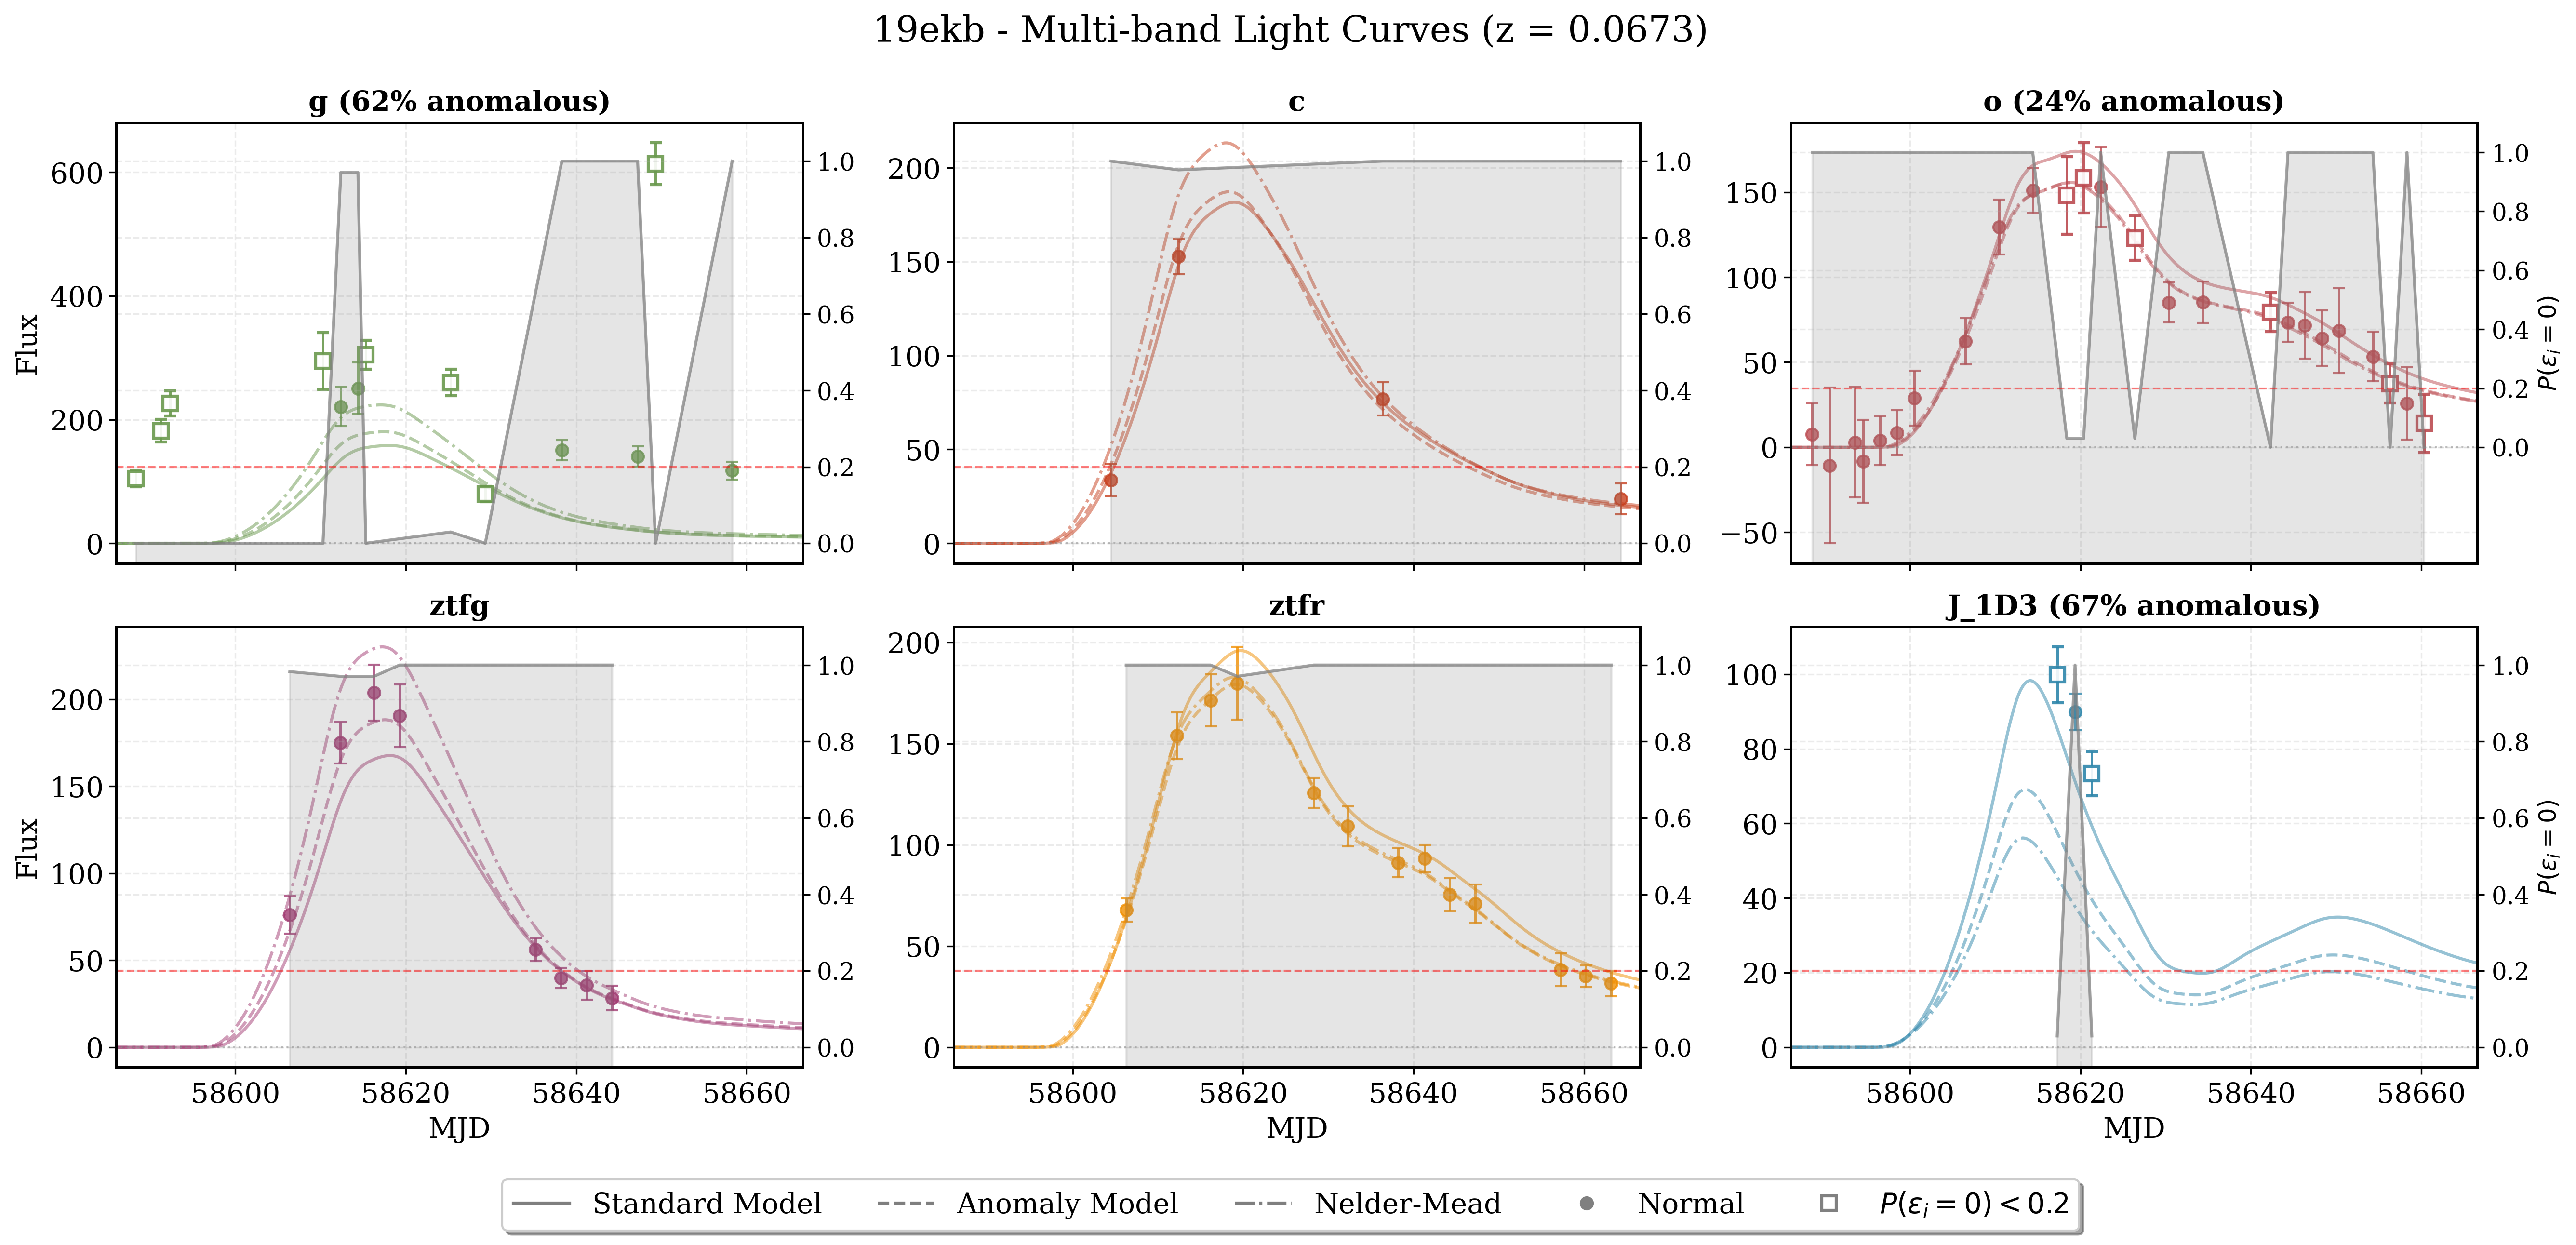
\includegraphics[width=\textwidth]{images/19ekb_light_curves_all_paper.png}
\caption{Light curve fits for SN 19ekb, with each panel showing a different transmission filter fit. All filters were fit jointly, then split up for visualisation only. Points that were likely to be anomalous (i.e., $P(\varepsilon=0) < 0.2$) are marked with squares. Other points are marked with dots. The grey line and shading represent the probability that each data point was anomalous, with the scale shown on the right-hand axis. The ZTF g band (green), which is ignored by traditional analysis, is partially preserved here.}
\label{fig:19ekb_lightcurves}
\end{figure*}

\subsection{SN 21hwx: Automatic Filter Removal and Identical Constraints}
\label{subsec:sn21hwx}

SN 21hwx presents a scenario where entire filters are systematically corrupted, demonstrating how the automated framework's decision aligns with manual analysis. The light curve in Figure~\ref{fig:21hwx_lightcurves} shows that the ZTF r, g, and j band data are entirely inconsistent with the supernova model.

The naive fit (Case A; Section~\ref{subsec:analysis_cases}) is strongly biased by these corrupted filters, producing skewed and unreliable parameter estimates. In our systematic filter selection (Case B; Section~\ref{subsec:analysis_cases}), these filters were identified and removed based on the $\chi^2$ criterion. Our framework (Case C; Section~\ref{subsec:analysis_cases}) arrives at the same conclusion automatically, flagging every data point in the ZTF r, g, and j bands as anomalous. Because both the systematic filter selection and anomaly detection methods effectively remove the same problematic data in this case, they produce statistically identical posterior constraints that are robust to the contaminating data, as shown in Figure~\ref{fig:21hwx_corner}. This case demonstrates the framework's capacity to automate this important data quality decision in a statistically principled and reproducible manner.

\begin{figure*}
\centering
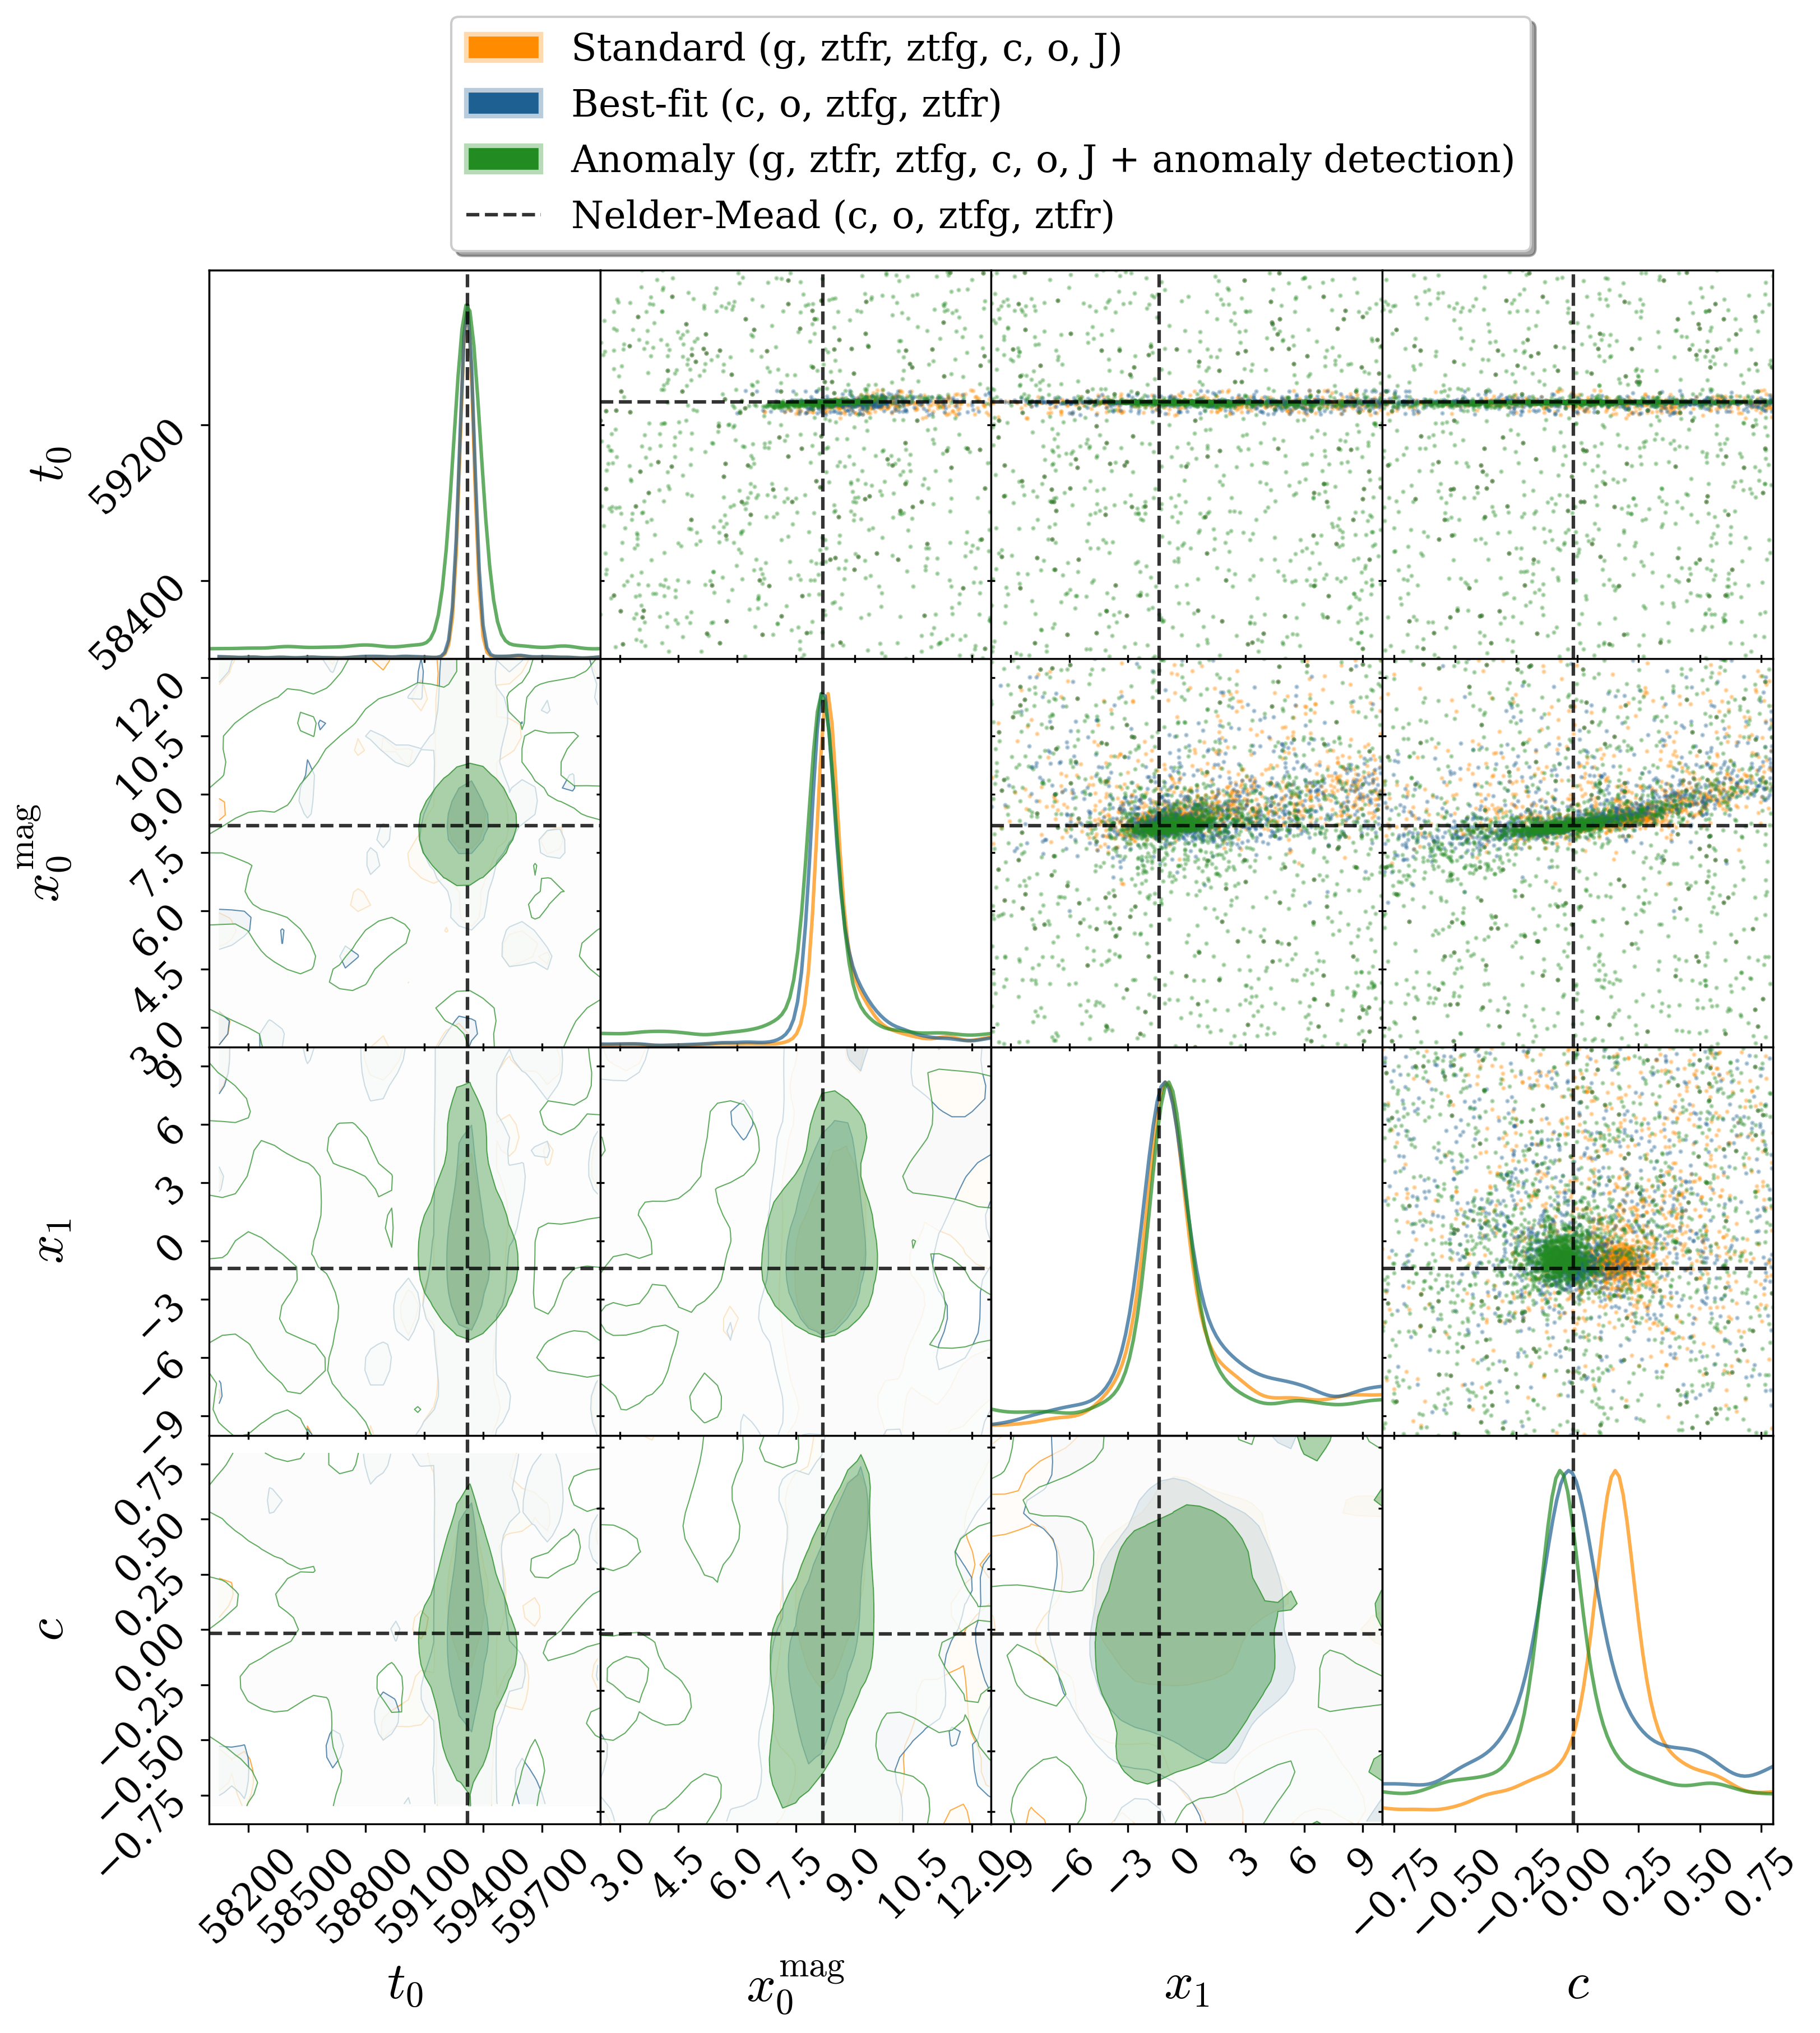
\includegraphics[width=0.8\textwidth]{images/corner_comparison_21hwx_paper_quality.png}
\caption{Corner plot showing posterior distributions for SN 21hwx across the three analysis methods (Cases A, B, and C; Section~\ref{subsec:analysis_cases}). The anomaly detection framework automatically identifies that the entire ZTF g and j bands require removal, matching the outcome from our systematic filter selection and yielding identical posterior constraints. The bands noted in each legend indicate the filters that were used in the fit.}
\label{fig:21hwx_corner}
\end{figure*}

\begin{figure*}
\centering
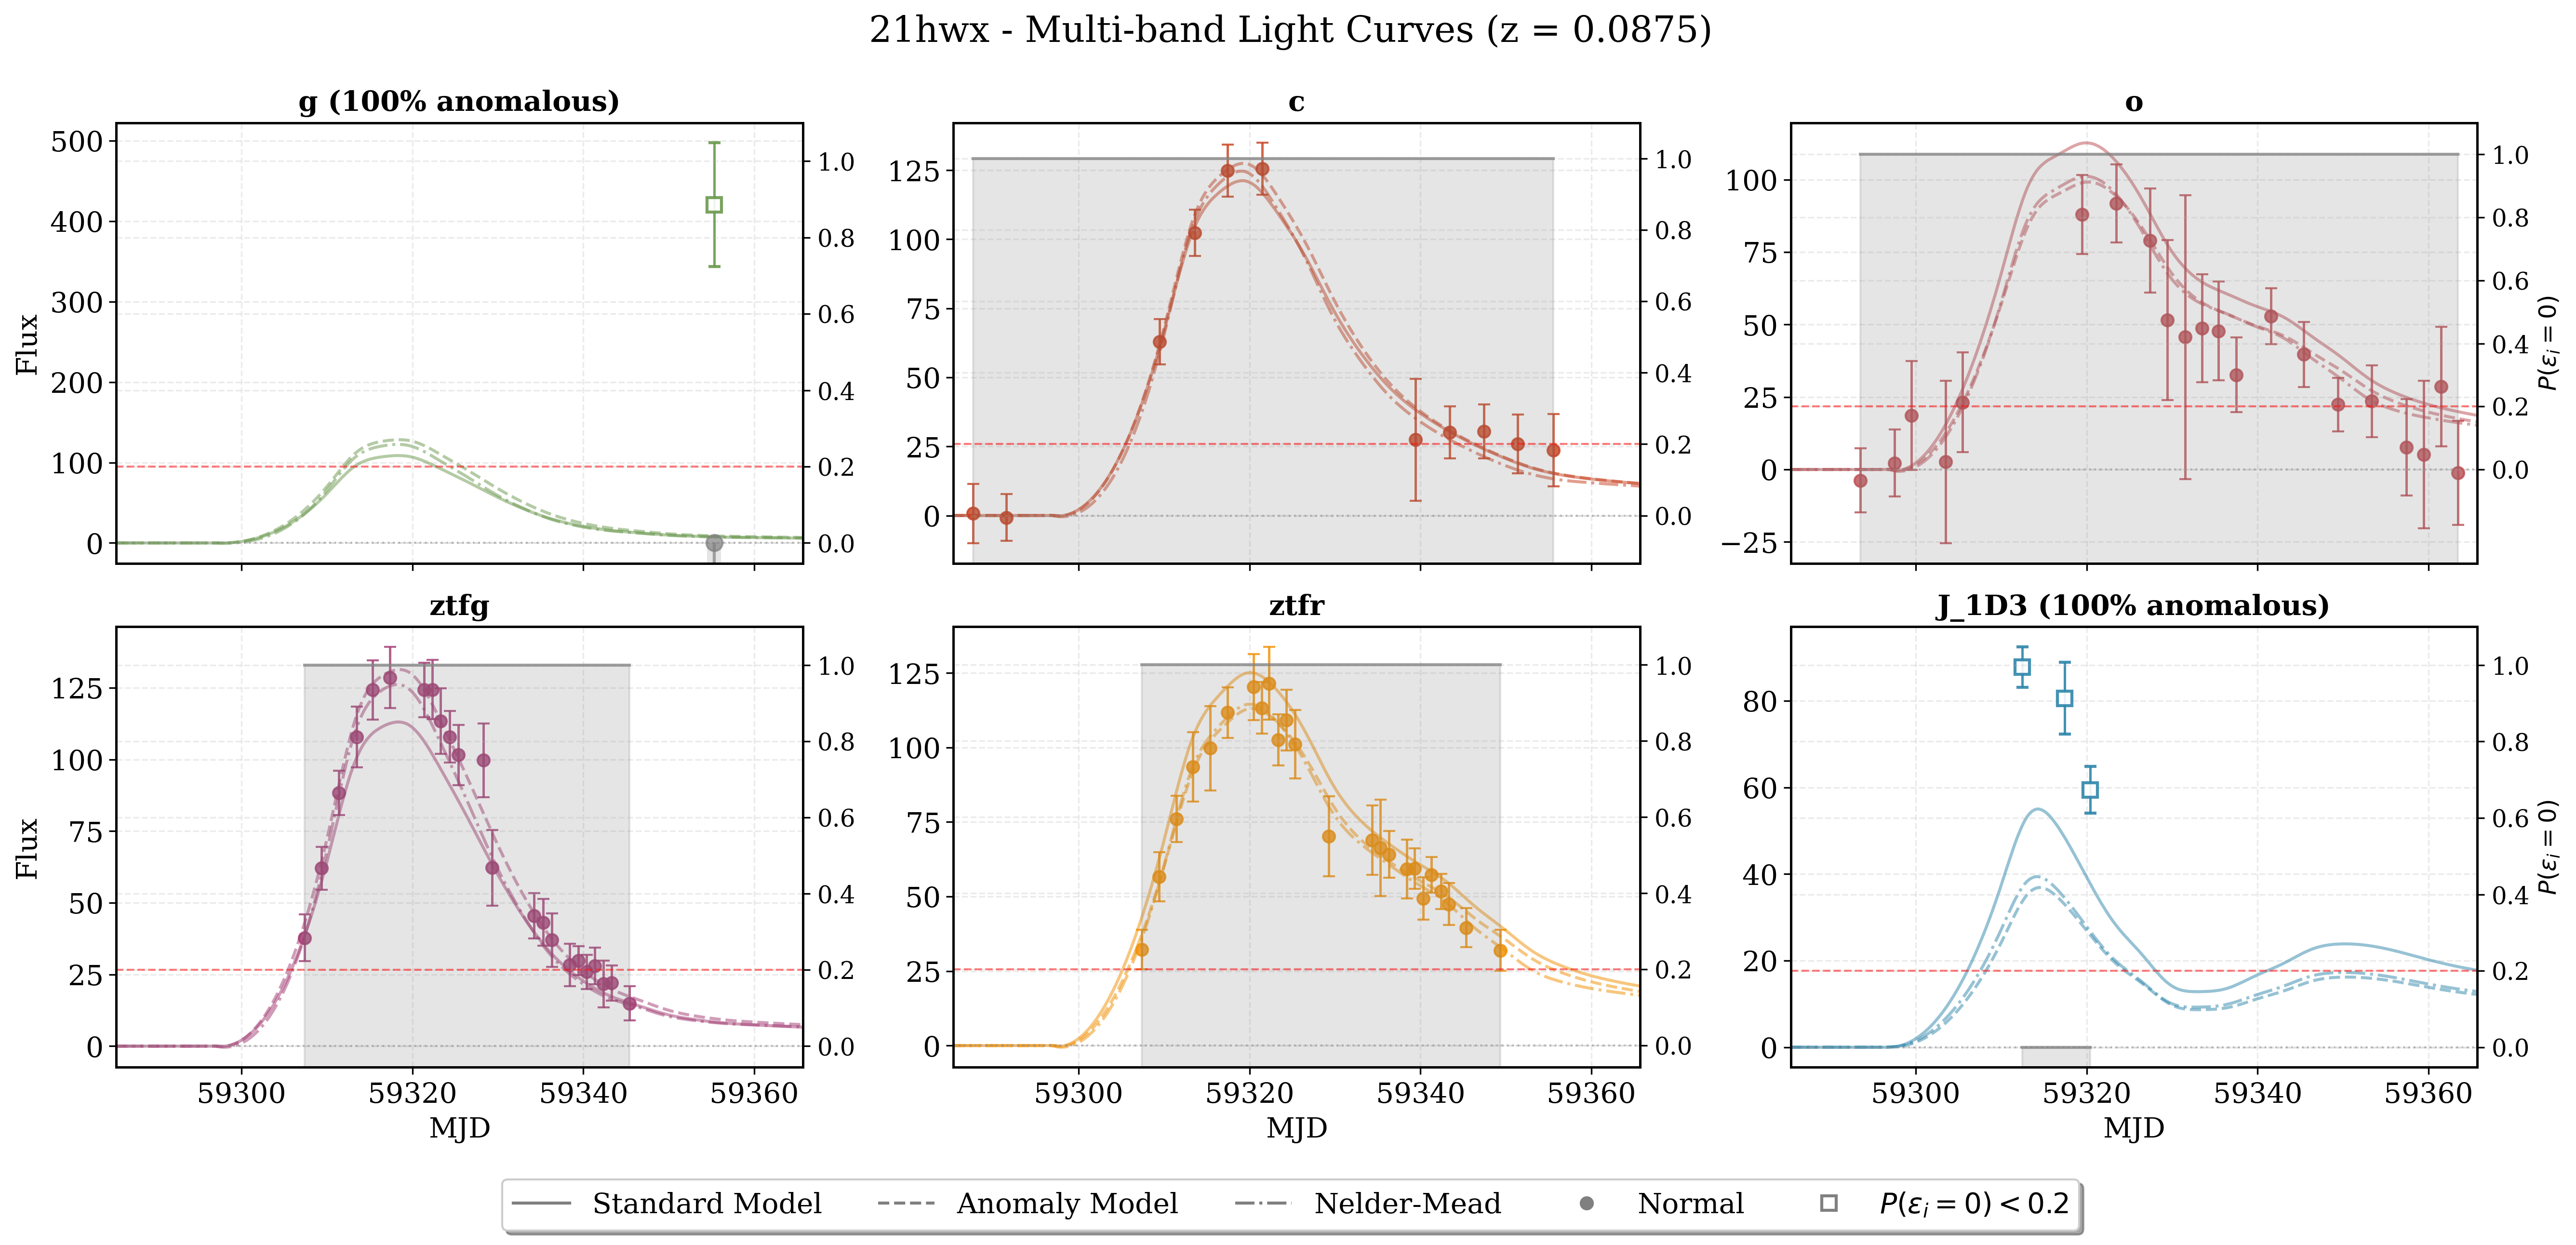
\includegraphics[width=\textwidth]{images/21hwx_light_curves_all_paper.png}
\caption{Light curve fits for SN 21hwx showing the anomaly detection framework automatically flags all points in the problematic ZTF g and j bands, matching the systematic removal of these filters in the traditional method. The grey line and shading represent the probability that each data point was anomalous, with the scale shown on the right-hand axis.}
\label{fig:21hwx_lightcurves}
\end{figure*}

\subsection{SN 21lnf: Selective Outlier Mitigation}
\label{subsec:sn21lnf}

The final example, SN 21lnf, represents a case with sporadic outliers scattered across multiple filters. As shown in the light curve plot (Figure~\ref{fig:21lnf_lightcurves}), the framework identifies and flags these individual anomalous points while preserving the surrounding data. A naive fit (Case A; Section~\ref{subsec:analysis_cases}) would be subtly biased by these points, while traditional filter selection approaches (Case B; Section~\ref{subsec:analysis_cases}) typically operate at the filter level rather than identifying individual outliers.

The posterior distributions in Figure~\ref{fig:21lnf_corner} show close agreement between the systematic filter selection and our automated framework, indicating that both methods converge on a similar result free from the influence of obvious outliers. However, the objective flagging of several low-significance outliers by our framework results in a minor but systematic shift in the posterior for the colour parameter, $c$. This highlights the framework's ability to correct for low-level systematic errors introduced by contaminated data points that can be missed by traditional, filter-level analyses. The framework achieves this outcome through an automated process, which is a desirable property for ensuring consistency and scalability in large surveys.

\begin{figure*}
\centering
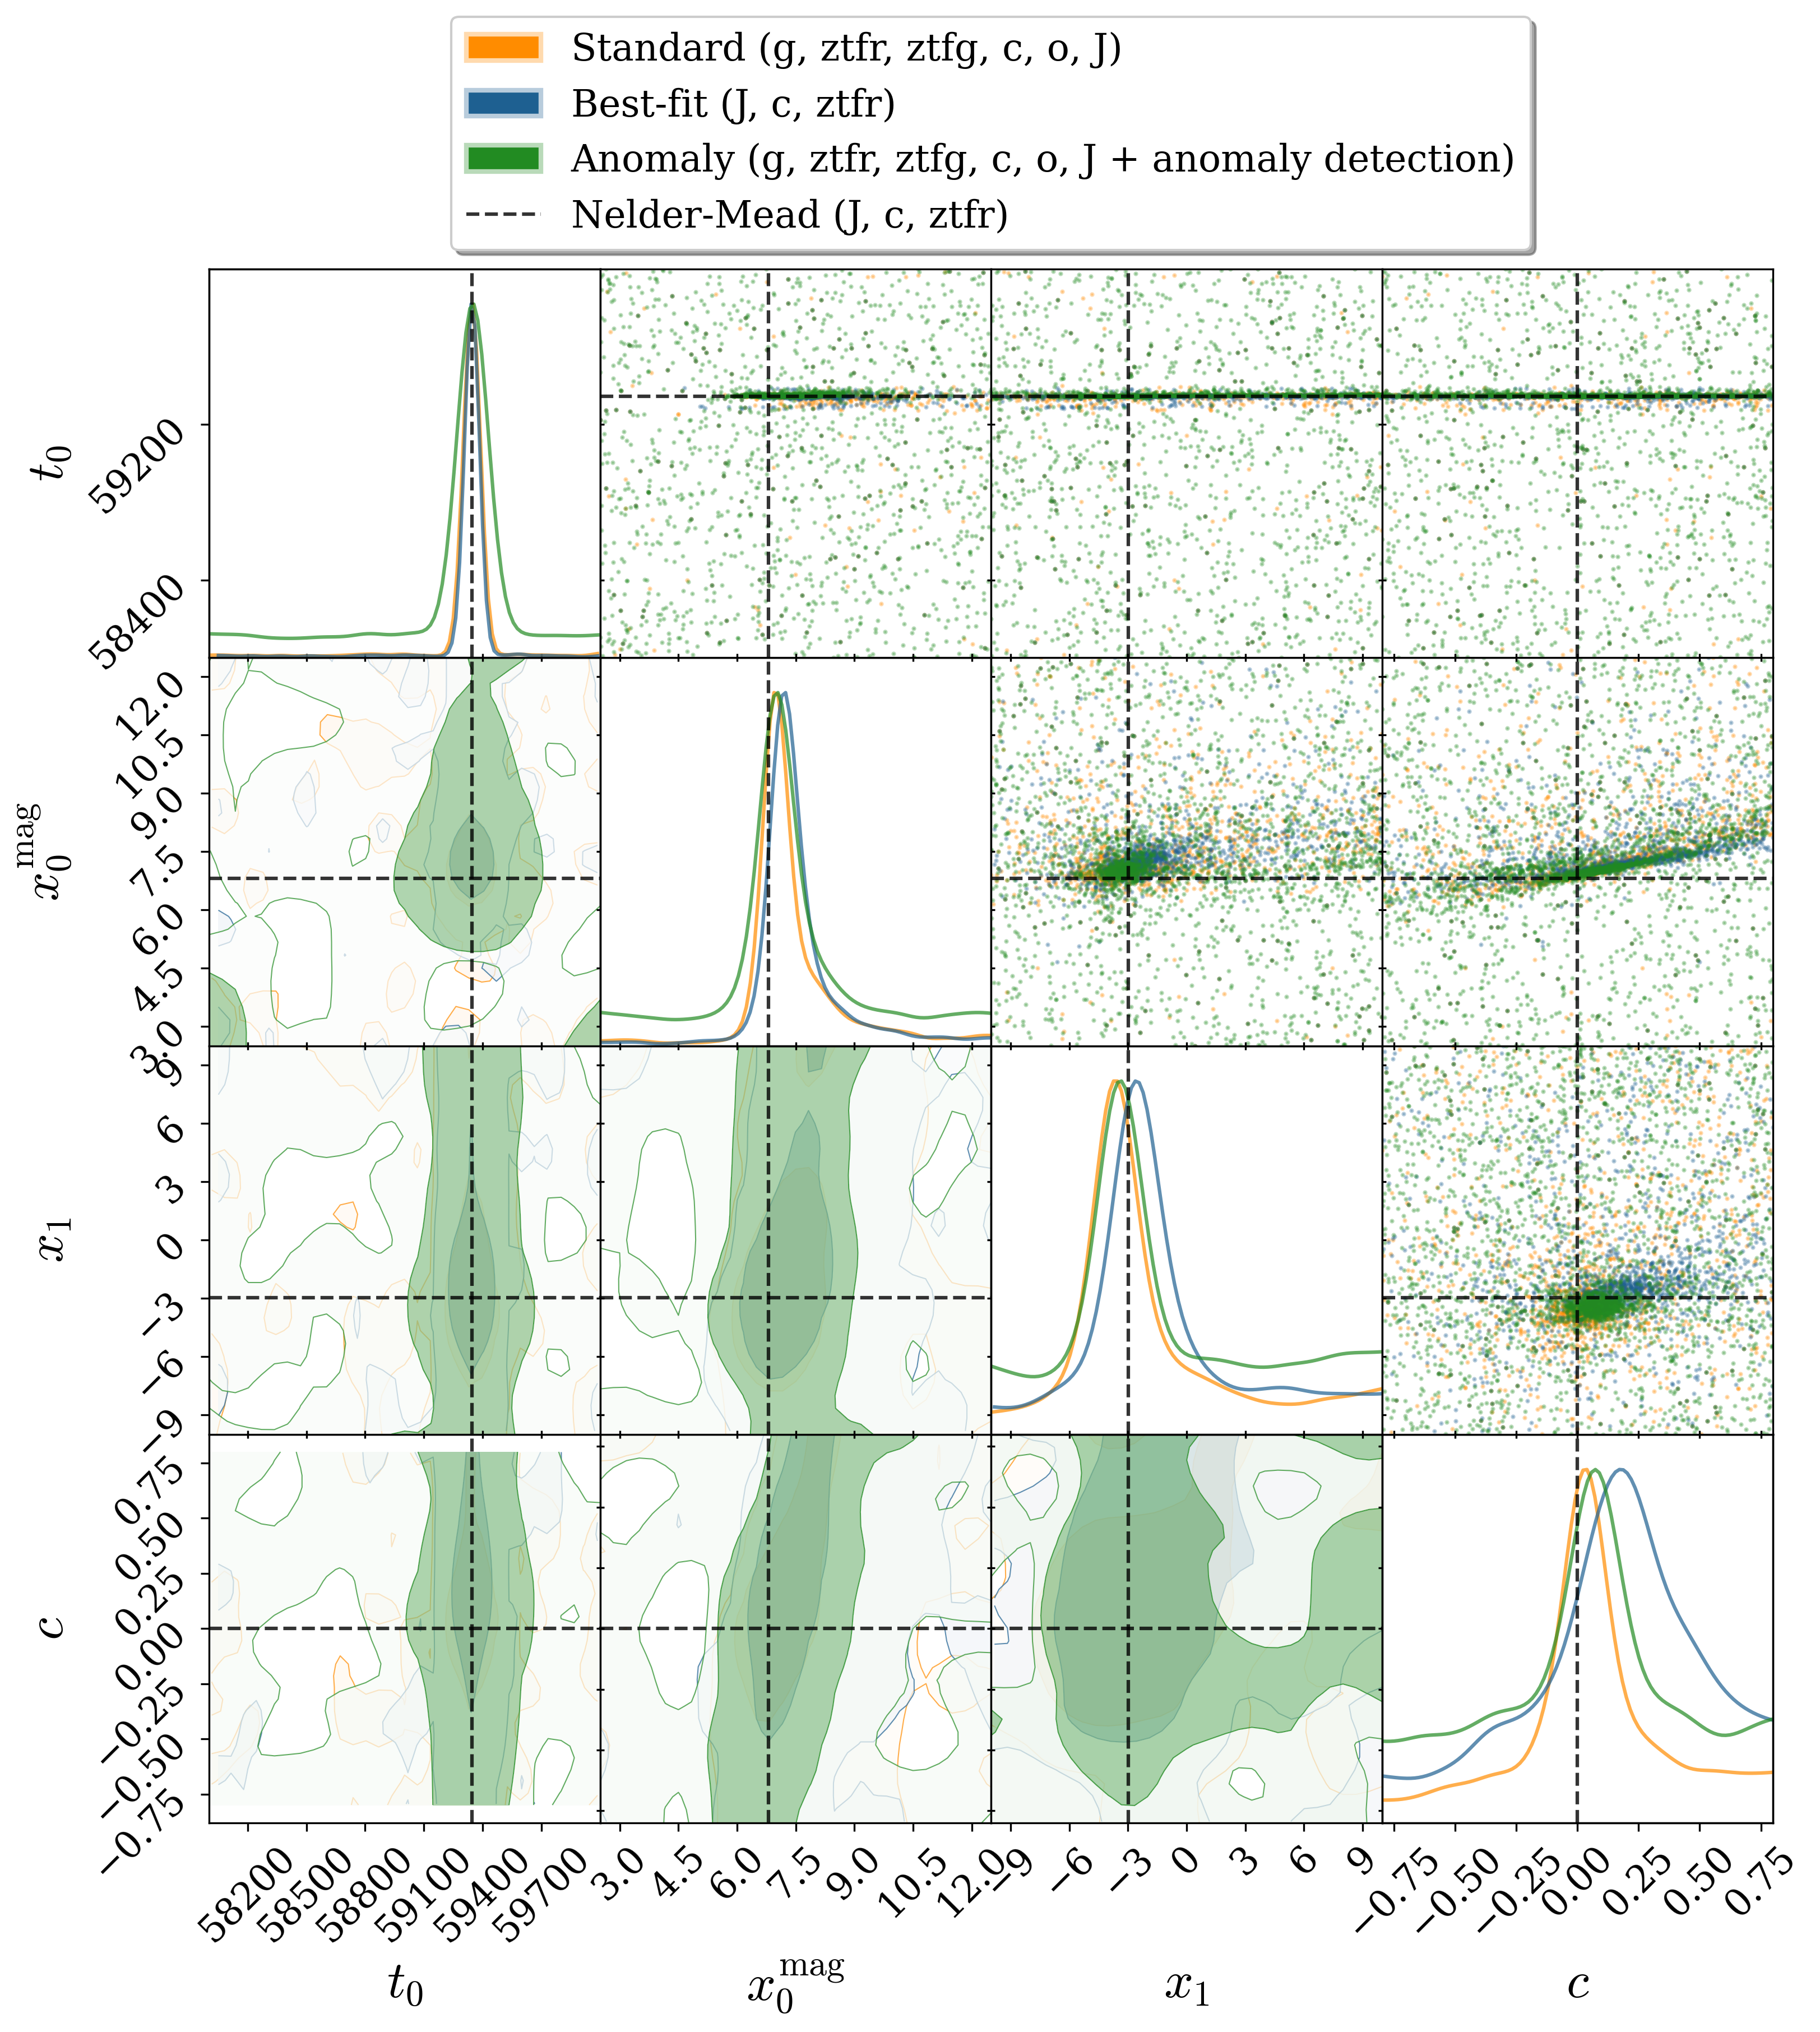
\includegraphics[width=0.8\textwidth]{images/corner_comparison_21lnf_paper_quality.png}
\caption{Corner plot showing posterior distributions for SALT parameters for SN 21lnf across the three analysis methods (Cases A, B, and C; Section~\ref{subsec:analysis_cases}). The systematic filter selection and anomaly detection framework produce consistent parameter estimates, demonstrating the framework's ability to identify sporadic outliers.}
\label{fig:21lnf_corner}
\end{figure*}

\begin{figure*}
\centering
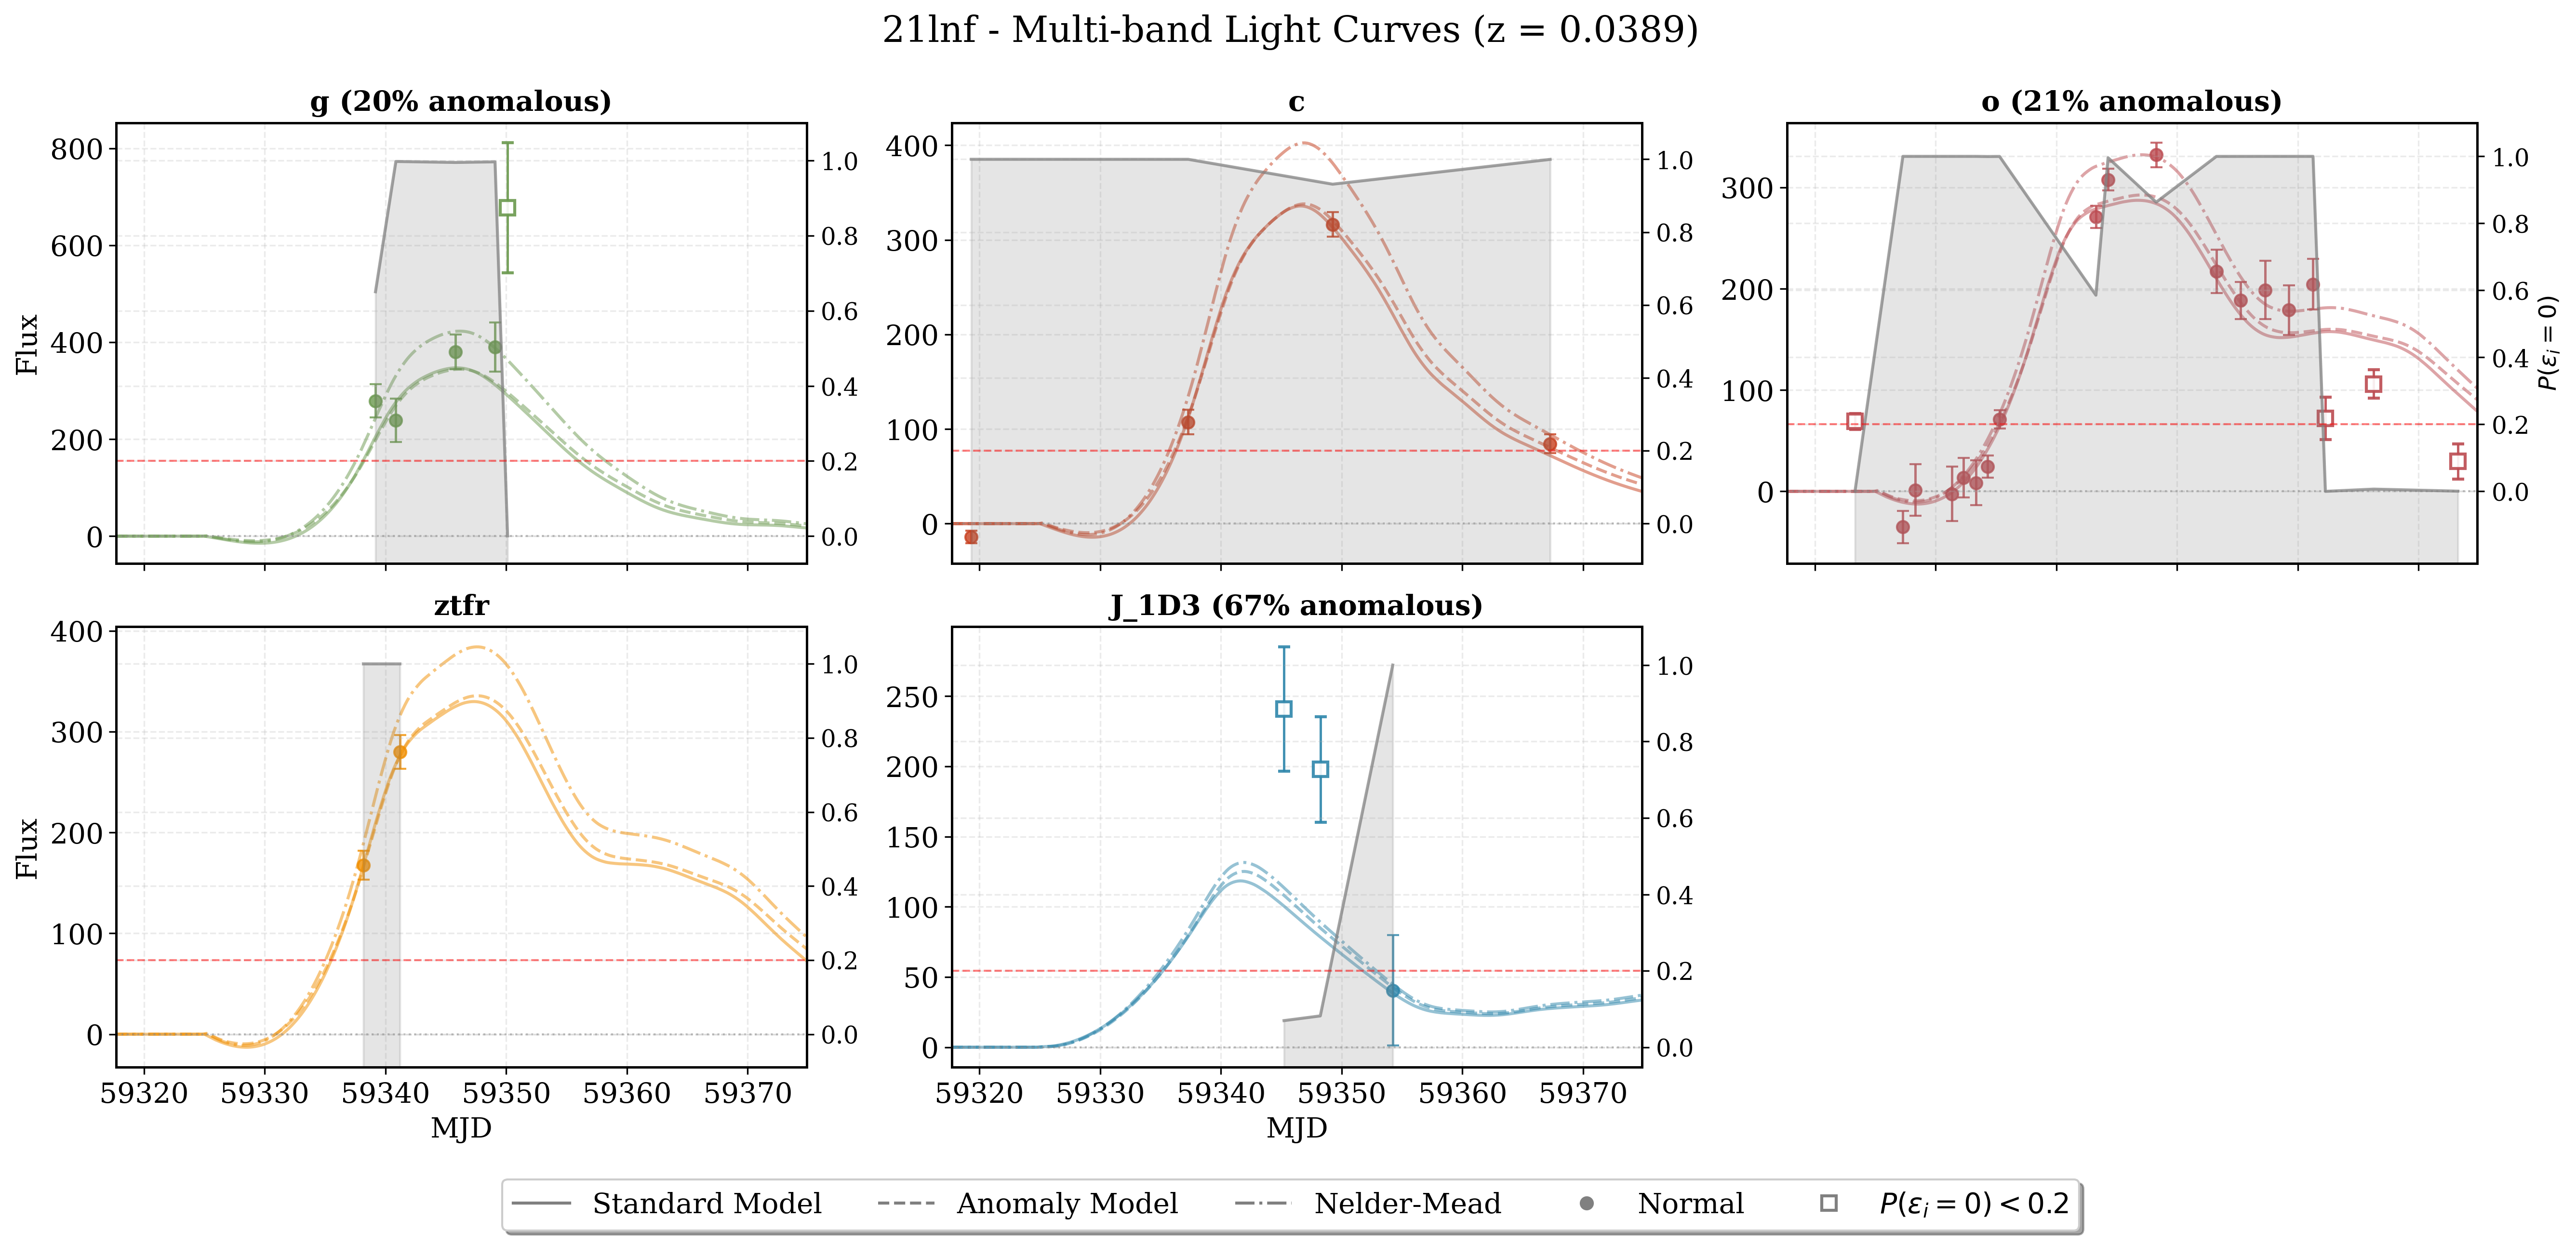
\includegraphics[width=\textwidth]{images/21lnf_light_curves_all_paper.png}
\caption{Light curve fits for SN 21lnf showing selective flagging of individual outliers across multiple bands. The anomaly detection identifies specific problematic measurements marked as squares while retaining all valid data marked as dots. The grey line and shading represent the probability that each data point was anomalous, with the scale shown on the right-hand axis.}
\label{fig:21lnf_lightcurves}
\end{figure*}